\documentclass{beamer}
\usepackage{graphicx} % Required for inserting images
\usepackage{appendix}
\usepackage{subfiles}
\usepackage{amsmath,amsthm,amssymb,latexsym} 
% For including math equations, theorems, symbols, etc
\usepackage{todonotes,comment,xr,hyperref,xcolor}


%%%%%%%%%%%%%%%%%%%%%%% NATURAL NUMBERS, INTEGERS, ETC. %%%%%%%%%%%%%%%%
\providecommand{\R}{}
\providecommand{\Z}{}
\providecommand{\N}{}
\providecommand{\C}{}
\providecommand{\Q}{}
\providecommand{\G}{}
\providecommand{\Lt}{}
\renewcommand{\R}{\mathbb{R}}
\renewcommand{\Z}{\mathbb{Z}}
\renewcommand{\N}{{\mathbb N}}
\renewcommand{\C}{\mathbb{C}}
\renewcommand{\Q}{\mathbb{Q}}
\renewcommand{\G}{\mathbb{G}}
\renewcommand{\Lt}{\mathbb{L}}
%%%%%%%%%%%%%%%%%%%%%%%%%%%%%%%%%%%%%%%%%%%%%%%%%%%%%

%%%%%%%%%%%%%%% BASIC PROBABILITY %%%%%%%%%%%%%%%%%%%%%%%%%%%%
\newcommand{\E}[1]{{\mathbf E}\left[#1\right]}										

\newcommand{\e}{{\mathbf E}}


\newcommand{\V}[1]{{\mathbf{Var}}\left\{#1\right\}}
\newcommand{\va}{{\mathbf{Var}}}
\newcommand{\p}[1]{{\mathbf P}\left\{#1\right\}}
\newcommand{\psub}[2]{{\mathbf P}_{#1}\left\{#2\right\}}
\newcommand{\psup}[2]{{\mathbf P}^{#1}\left\{#2\right\}}
\newcommand{\I}[1]{{\mathbf 1}_{[#1]}}
\newcommand{\set}[1]{\left\{ #1 \right\}}
% \Cprob Bases bracket size on term before conditioning; \probC on term after conditioning
\newcommand{\Cprob}[2]{\mathbf{P}\set{\left. #1 \; \right| \; #2}} 
\newcommand{\probC}[2]{\mathbf{P}\set{#1 \; \left|  \; #2 \right. }}
\newcommand{\phat}[1]{\ensuremath{\hat{\mathbf P}}\left\{#1\right\}}
\newcommand{\Ehat}[1]{\ensuremath{\hat{\mathbf E}}\left[#1\right]}
\newcommand{\ehat}{\ensuremath{\hat{\mathbf E}}}
\newcommand{\Esup}[2]{{\mathbf E^{#1}}\left\{#2\right\}}
\newcommand{\esup}[1]{{\mathbf E^{#1}}}
\newcommand{\Esub}[2]{{\mathbf E_{#1}}\left\{#2\right\}}
\newcommand{\esub}[1]{{\mathbf E_{#1}}}
%%%%%%%%%%%%%%%%%%%%%%%%%%%%%%%%%%%%%%%%%%%%%%%%%%%%%

%%%%%%%%%%%%%%%%%%%%%%%%%%%%% SETS %%%%%%%%%%%%%%%%%%%%%
\newcommand\cA{\mathcal A}
\newcommand\cB{\mathcal B}
\newcommand\cC{\mathcal C}
\newcommand\cD{\mathcal D}
\newcommand\cE{\mathcal E}
\newcommand\cF{\mathcal F}
\newcommand\cG{\mathcal G}
\newcommand\cH{\mathcal H}
\newcommand\cI{\mathcal I}
\newcommand\cJ{\mathcal J}
\newcommand\cK{\mathcal K}
\newcommand\cL{{\mathcal L}}
\newcommand\cM{\mathcal M}
\newcommand\cN{\mathcal N}
\newcommand\cO{\mathcal O}
\newcommand\cP{\mathcal P}
\newcommand\cQ{\mathcal Q}
\newcommand\cR{{\mathcal R}}
\newcommand\cS{{\mathcal S}}
\newcommand\cT{{\mathcal T}}
\newcommand\cU{{\mathcal U}}
\newcommand\cV{\mathcal V}
\newcommand\cW{\mathcal W}
\newcommand\cX{{\mathcal X}}
\newcommand\cY{{\mathcal Y}}
\newcommand\cZ{{\mathcal Z}}
%%%%%%%%%%%%%%%%%%%%%%%%%%%%%%%%%%%%%%%%%%%%%%%%%%%%%%

%%%%%%%%%%%%%%%%%%%%%%%%%%%%% BOLDFACE %%%%%%%%%%%%%%%%%%%%
\newcommand{\bA}{\mathbf{A}} 
\newcommand{\bB}{\mathbf{B}} 
\newcommand{\bC}{\mathbf{C}} 
\newcommand{\bD}{\mathbf{D}} 
\newcommand{\bE}{\mathbf{E}} 
\newcommand{\bF}{\mathbf{F}} 
\newcommand{\bG}{\mathbf{G}} 
\newcommand{\bH}{\mathbf{H}} 
\newcommand{\bI}{\mathbf{I}} 
\newcommand{\bJ}{\mathbf{J}} 
\newcommand{\bK}{\mathbf{K}} 
\newcommand{\bL}{\mathbf{L}} 
\newcommand{\bM}{\mathbf{M}} 
\newcommand{\bN}{\mathbf{N}} 
\newcommand{\bO}{\mathbf{O}} 
\newcommand{\bP}{\mathbf{P}} 
\newcommand{\bQ}{\mathbf{Q}} 
\newcommand{\bR}{\mathbf{R}} 
\newcommand{\bS}{\mathbf{S}} 
\newcommand{\bT}{\mathbf{T}} 
\newcommand{\bU}{\mathbf{U}} 
\newcommand{\bV}{\mathbf{V}} 
\newcommand{\bW}{\mathbf{W}} 
\newcommand{\bX}{\mathbf{X}} 
\newcommand{\bY}{\mathbf{Y}} 
\newcommand{\bZ}{\mathbf{Z}}
%%%%%%%%%%%%%%%%%%%%%%%%%%%%%%%%%%%%%%%%%%%%%%%%%%%%%%%%

%%%%%%%%%%%%%%% PROBABILISTIC CONVERGENCE/EQUALITY %%%%%%%%%%%%%%%%%%%%%%%
\newcommand{\eqdist}{\ensuremath{\stackrel{\mathrm{d}}{=}}}
\newcommand{\convdist}{\ensuremath{\stackrel{\mathrm{d}}{\rightarrow}}}
\newcommand{\convas}{\ensuremath{\stackrel{\mathrm{a.s.}}{\rightarrow}}}
\newcommand{\aseq}{\ensuremath{\stackrel{\mathrm{a.s.}}{=}}}


%%%%%%%%%%%%%%%%%%%%%%% Theorem types %%%%%%%%%%%%%%%%%
\newtheorem{thm}{Theorem}[section]
\newtheorem{lem}[thm]{Lemma}
\newtheorem{prop}[thm]{Proposition}
\newtheorem{cor}[thm]{Corollary}
\newtheorem{dfn}[thm]{Definition}
\newtheorem{conj}{Conjecture}
\newtheorem{ex}{Exercise}[section]
\newtheorem{claim}[thm]{Claim}
\newtheorem{cla}[thm]{Claim}
\newtheorem{remark}[thm]{Remark}
\newtheorem{hyp}[thm]{Hypothesis}
\newtheorem{notation}[thm]{Notation}
\endinput
\usepackage{multimedia}
\usepackage{media9}

\usetheme{AnnArbor}
\title{Branching Brownian motion and Fisher-KPP}
\author{Leo Tyrpak}
\institute{Oxford}
\date{February 2025}

\begin{document}
\maketitle
\begin{comment}
    Be less general, take easy parameters.
\end{comment}
\begin{comment}
    Abstract:
    In this presentation we will introduce the model given in 'Looking forwards and backwards: dynamics and genealogies of locally regulated populations' by Etheridge et al.
    This is an individual based spatial birth and death process where the main parameters birth and death depend on the population as a whole.
    This will be a gentle introduction to how the model is defined, what it models, scaling limits and characterisation of flcutuations when the scaling limit is deterministic.
\end{comment}

\begin{frame}{Contents}
\begin{itemize}
    \item Brownian motion
    \item Relation Brownian motion and heat equation
    \item Branching processes
    \item Branching Brownian motion
    \item Fisher-KPP
\end{itemize}
    
\end{frame}



\begin{frame}{Brownian motion in 1d}
    
\end{frame}


\begin{frame}{Brownian Motion in 2D}
    
\end{frame}



\begin{frame}{Definition of BM}
\begin{thm}[CLT]
    Let $X_1,...,X_n$ i.i.d. with $\E{X_1}=0,\E{X_1^2}=1$ then $\frac{X_1+...+X_n}{\sqrt{n}}\rightarrow^d\cN$ where $\cN$ is a standard normal.
\end{thm}
    \begin{itemize}
        \item Describes random motion of particles in a medium
        \item Let $X_1,...,X_n,..$ i.i.d with $\E{X_1}=0,\E{X_1^2}=1$, e.g. $X_1=2\text{Ber}(1/2)-1$
        \item Define $S^n_t=\sum_{i=1}^{\lfloor tn\rfloor}X_i$
        \item Donsker Invariance: $(\frac{1}{\sqrt{n}}S^n(t))_{n\geq0}$ converges to $B_t$ standard Brownian motion
        \item Used to simulate BBM in practice
    \end{itemize}
    
\end{frame}


\begin{frame}{Connection to PDE}
    \begin{thm}[Feynman-Kac formula]
        Let $u(t,x)$ be the unique solution to heat equation $u(0,x)=g(x)$ and $\partial_t u=\frac{1}{2}\Delta u$ then $u(t,x)=\E{g(W_t+x)|W=0}$.
    \end{thm}
    \begin{itemize}
        \item $(B_t)_{t\geq0}$ is a random path
        \item Direct check, $B_t\sim^d\cN(0,t)$ so has density $G_t(x,y)=\frac{1}{\sqrt{2\pi t}}\exp{(-\frac{(x-y)^2}{2t})}$
        \item Solution $u(t,x)=\int_{\R^d}G_t(x,y)g(y)dy$
        \item Solve PDE by simulating BM (Monte Carlo)
    \end{itemize}
\end{frame}

\begin{frame}{Sketch proof}
    \begin{itemize}
        \item Show $u_n(t,x)=\E{g(\frac{1}{\sqrt{n}}S^n_t+x)}$ satisfies $\partial_tu_n\approx\frac{1}{2}\Delta u_n$, $d=1$
        \item $\frac{1}{2}\Delta u_n=\frac{1}{2}\E{g''(\frac{1}{\sqrt{n}}S^n_t+x)}$
        \item Taylor expansion:
        \begin{align*}
            u_n(t+\frac{1}{n},x)
            &=\E{g(\frac{1}{\sqrt{n}}S^n_t+\frac{1}{\sqrt{n}}X_{\lfloor nt\rfloor+1}+x)}\\
            &\approx\E{g(\frac{1}{\sqrt{n}}S^n_t+x)}+\E{(\frac{1}{\sqrt{n}}X_{\lfloor nt\rfloor+1})g'(\frac{1}{\sqrt{n}}S^n_t+x)}\\
            &+\frac{1}{2}\E{(\frac{1}{\sqrt{n}}X_{\lfloor nt\rfloor+1})^2g''(\frac{1}{\sqrt{n}}S^n_t+x)}\\
            &=u_n(t,x)+0+\frac{1}{2n}\Delta u_n(t,x)
        \end{align*}
        \item Therefore $\frac{u_n(t+\frac{1}{n},x)-u(t,x)}{n}=\frac{1}{2}\Delta u(t,x)$
        \item Generalises to linear evolution equation $\partial_t u=Au$
    \end{itemize}
\end{frame}


\begin{frame}{Branching}
    \begin{figure}
        \centering
        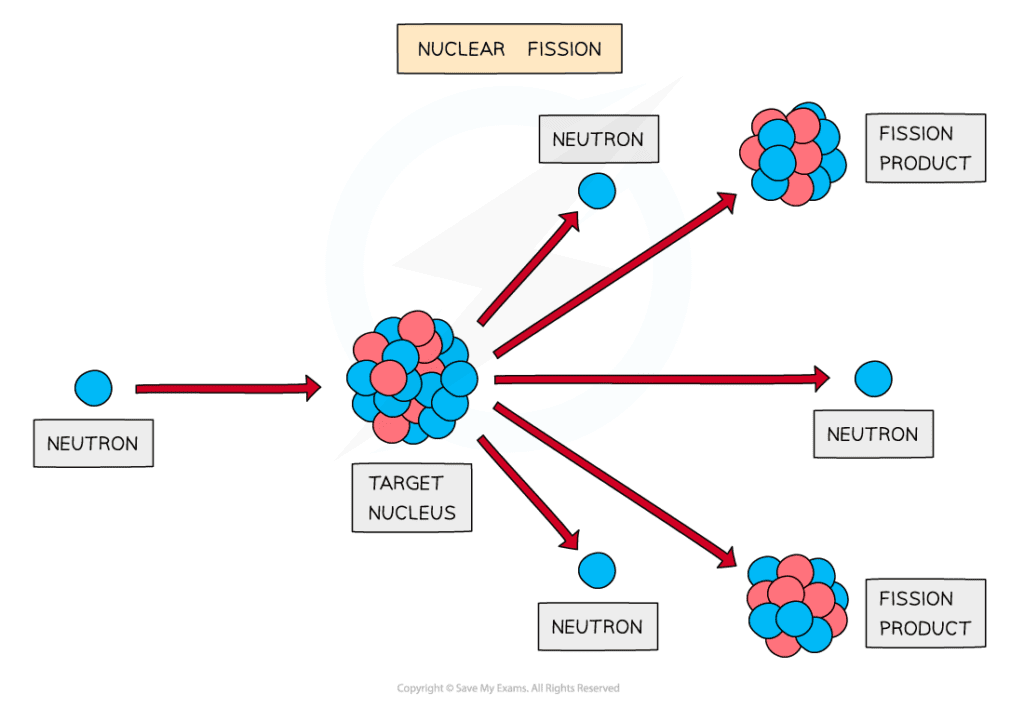
\includegraphics[width=0.8\linewidth]{branching BM/fission.png}
        \caption{Branching from fission}
        \label{fig:enter-label}
    \end{figure}
\end{frame}


\begin{frame}{Branching processes}
    \begin{itemize}
        \item Counts $N_t=$\#bacteria at time $t$
        \item $N_0=1$, each bacteria divides in $2$ after waiting $\text{Exp}(1)$ random variable
        \item After division, $2$ bacteria evolve independently
        \item Can model populations reproducing, fission in nuclear reactors, etc
        \item Called Yule process, Check $\E{N_t}=\exp t$
    \end{itemize}
\end{frame}


\begin{frame}{Branching BM simulation}
    
\end{frame}


\begin{frame}{Branching BM}
    \begin{itemize}
        \item Start with $1$ particle time $0$
        \item Each particle moves as BM
        \item After $\text{Exp}(1)$, split in 2
        \item Each child evolves independently as branching BM
        \item $N_t$=\# particles is Yule process
    \end{itemize}
\end{frame}


\begin{frame}{Fisher-KPP}
    \begin{itemize}
        \item Consider the equation $\partial_tu=\frac{1}{2}\Delta u+u(1-u)$, $u(0,x)=g(x)$
        \item Used to model population growth
        \item Capacity $1$, diffusion from $\Delta$ and growth rate $u-1$
        \item Stationary solutions; $u\equiv1$ stable, $u\equiv0$ unstable
        \item Observation: Convergence to travelling wave
        \item Travelling wave speed $c$ form $u(t,x)=w(x-ct)$
        \item Satisfies $\frac{1}{2}w''+cw'+w(1-w)=0$
    \end{itemize}
\end{frame}


\begin{frame}{Traveling wave}
    \begin{itemize}
        \item First result, Kolmogorov-Petrovsky-Piscounov: $\exists m_t$ such that $u(t,x+m_t)\rightarrow w(x)$ as $t\rightarrow\infty$ uniformly in $x$
        \item Furthermore $m_t=\sqrt{2}t+o(t)$ and $\frac{1}{2}w''+\sqrt{2}w'+w(1-w)=0$
        \item McKean representation: $u(t,x)=1-\E{\prod_{i=1}^{N_t}(1-g(X_i(t)+x))}$
        \item where $X_i$ are location of particles in BBM, $N_t$ number of particles
        \item Elegant proof using martingales
        \item Usually $g(x)=1_{x\leq0}$
        \item Then $u(t,x)=1-\p{X_i(t)>-x: \forall 1\leq i\leq N_t}=\p{X_i(t)>x: \exists 1\leq i\leq N_t}$
        \item So $u(t,x)=\p{\max(X_i(t))>x}$
    \end{itemize}
    
\end{frame}


\begin{frame}{First moment estimates}
    \begin{align*}
        u(t,ct)&=\p{\exists 1\leq i\leq N_t, X_i(t)>ct}\\
        &\leq\E{\sum_i1_{X_i(t)>ct}}\\
        &=e^t\p{B(t)>ct}=e^t\p{\cN>c\sqrt{t}}\\
        &\leq De^t\frac{\exp{(-c^2t/2)}}{c\sqrt{2\pi t}}= D\exp{(t(1-c^2/2))}\frac{1}{c\sqrt{2\pi t}}
    \end{align*}
    Therefore for $c\geq\sqrt{2}$ this tends to $0$\\
    One can also show the first moment tends to $\infty$ if $c<\sqrt{2}$, need that probability is then close to first moment.
\end{frame}

\end{document}